\documentclass[1p]{elsarticle_modified}
%\bibliographystyle{elsarticle-num}

%\usepackage[colorlinks]{hyperref}
%\usepackage{abbrmath_seonhwa} %\Abb, \Ascr, \Acal ,\Abf, \Afrak
\usepackage{amsfonts}
\usepackage{amssymb}
\usepackage{amsmath}
\usepackage{amsthm}
\usepackage{scalefnt}
\usepackage{amsbsy}
\usepackage{kotex}
\usepackage{caption}
\usepackage{subfig}
\usepackage{color}
\usepackage{graphicx}
\usepackage{xcolor} %% white, black, red, green, blue, cyan, magenta, yellow
\usepackage{float}
\usepackage{setspace}
\usepackage{hyperref}

\usepackage{tikz}
\usetikzlibrary{arrows}

\usepackage{multirow}
\usepackage{array} % fixed length table
\usepackage{hhline}

%%%%%%%%%%%%%%%%%%%%%
\makeatletter
\renewcommand*\env@matrix[1][\arraystretch]{%
	\edef\arraystretch{#1}%
	\hskip -\arraycolsep
	\let\@ifnextchar\new@ifnextchar
	\array{*\c@MaxMatrixCols c}}
\makeatother %https://tex.stackexchange.com/questions/14071/how-can-i-increase-the-line-spacing-in-a-matrix
%%%%%%%%%%%%%%%

\usepackage[normalem]{ulem}

\newcommand{\msout}[1]{\ifmmode\text{\sout{\ensuremath{#1}}}\else\sout{#1}\fi}
%SOURCE: \msout is \stkout macro in https://tex.stackexchange.com/questions/20609/strikeout-in-math-mode

\newcommand{\cancel}[1]{
	\ifmmode
	{\color{red}\msout{#1}}
	\else
	{\color{red}\sout{#1}}
	\fi
}

\newcommand{\add}[1]{
	{\color{blue}\uwave{#1}}
}

\newcommand{\replace}[2]{
	\ifmmode
	{\color{red}\msout{#1}}{\color{blue}\uwave{#2}}
	\else
	{\color{red}\sout{#1}}{\color{blue}\uwave{#2}}
	\fi
}

\newcommand{\Sol}{\mathcal{S}} %segment
\newcommand{\D}{D} %diagram
\newcommand{\A}{\mathcal{A}} %arc


%%%%%%%%%%%%%%%%%%%%%%%%%%%%%5 test

\def\sl{\operatorname{\textup{SL}}(2,\Cbb)}
\def\psl{\operatorname{\textup{PSL}}(2,\Cbb)}
\def\quan{\mkern 1mu \triangleright \mkern 1mu}

\theoremstyle{definition}
\newtheorem{thm}{Theorem}[section]
\newtheorem{prop}[thm]{Proposition}
\newtheorem{lem}[thm]{Lemma}
\newtheorem{ques}[thm]{Question}
\newtheorem{cor}[thm]{Corollary}
\newtheorem{defn}[thm]{Definition}
\newtheorem{exam}[thm]{Example}
\newtheorem{rmk}[thm]{Remark}
\newtheorem{alg}[thm]{Algorithm}

\newcommand{\I}{\sqrt{-1}}
\begin{document}

%\begin{frontmatter}
%
%\title{Boundary parabolic representations of knots up to 8 crossings}
%
%%% Group authors per affiliation:
%\author{Yunhi Cho} 
%\address{Department of Mathematics, University of Seoul, Seoul, Korea}
%\ead{yhcho@uos.ac.kr}
%
%
%\author{Seonhwa Kim} %\fnref{s_kim}}
%\address{Center for Geometry and Physics, Institute for Basic Science, Pohang, 37673, Korea}
%\ead{ryeona17@ibs.re.kr}
%
%\author{Hyuk Kim}
%\address{Department of Mathematical Sciences, Seoul National University, Seoul 08826, Korea}
%\ead{hyukkim@snu.ac.kr}
%
%\author{Seokbeom Yoon}
%\address{Department of Mathematical Sciences, Seoul National University, Seoul, 08826,  Korea}
%\ead{sbyoon15@snu.ac.kr}
%
%\begin{abstract}
%We find all boundary parabolic representation of knots up to 8 crossings.
%
%\end{abstract}
%\begin{keyword}
%    \MSC[2010] 57M25 
%\end{keyword}
%
%\end{frontmatter}

%\linenumbers
%\tableofcontents
%
\newcommand\colored[1]{\textcolor{white}{\rule[-0.35ex]{0.8em}{1.4ex}}\kern-0.8em\color{red} #1}%
%\newcommand\colored[1]{\textcolor{white}{ #1}\kern-2.17ex	\textcolor{white}{ #1}\kern-1.81ex	\textcolor{white}{ #1}\kern-2.15ex\color{red}#1	}

{\Large $\underline{12a_{1120}~(K12a_{1120})}$}

\setlength{\tabcolsep}{10pt}
\renewcommand{\arraystretch}{1.6}
\vspace{1cm}\begin{tabular}{m{100pt}>{\centering\arraybackslash}m{274pt}}
\multirow{5}{120pt}{
	\centering
	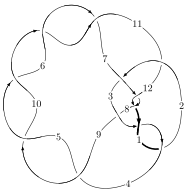
\includegraphics[width=112pt]{../../../GIT/diagram.site/Diagrams/png/1921_12a_1120.png}\\
\ \ \ A knot diagram\footnotemark}&
\allowdisplaybreaks
\textbf{Linearized knot diagam} \\
\cline{2-2}
 &
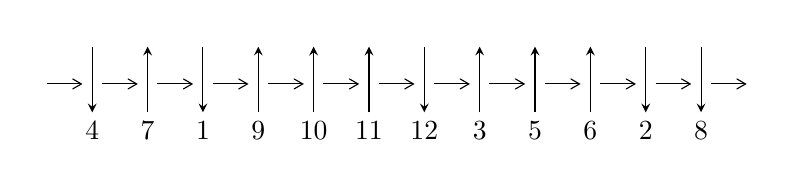
\begin{tikzpicture}[x=20pt, y=17pt]
	% nodes
	\node (C0) at (0, 0) {};
	\node (C1) at (1, 0) {};
	\node (C1U) at (1, +1) {};
	\node (C1D) at (1, -1) {4};

	\node (C2) at (2, 0) {};
	\node (C2U) at (2, +1) {};
	\node (C2D) at (2, -1) {7};

	\node (C3) at (3, 0) {};
	\node (C3U) at (3, +1) {};
	\node (C3D) at (3, -1) {1};

	\node (C4) at (4, 0) {};
	\node (C4U) at (4, +1) {};
	\node (C4D) at (4, -1) {9};

	\node (C5) at (5, 0) {};
	\node (C5U) at (5, +1) {};
	\node (C5D) at (5, -1) {10};

	\node (C6) at (6, 0) {};
	\node (C6U) at (6, +1) {};
	\node (C6D) at (6, -1) {11};

	\node (C7) at (7, 0) {};
	\node (C7U) at (7, +1) {};
	\node (C7D) at (7, -1) {12};

	\node (C8) at (8, 0) {};
	\node (C8U) at (8, +1) {};
	\node (C8D) at (8, -1) {3};

	\node (C9) at (9, 0) {};
	\node (C9U) at (9, +1) {};
	\node (C9D) at (9, -1) {5};

	\node (C10) at (10, 0) {};
	\node (C10U) at (10, +1) {};
	\node (C10D) at (10, -1) {6};

	\node (C11) at (11, 0) {};
	\node (C11U) at (11, +1) {};
	\node (C11D) at (11, -1) {2};

	\node (C12) at (12, 0) {};
	\node (C12U) at (12, +1) {};
	\node (C12D) at (12, -1) {8};
	\node (C13) at (13, 0) {};

	% arrows
	\draw[->,>={angle 60}]
	(C0) edge (C1) (C1) edge (C2) (C2) edge (C3) (C3) edge (C4) (C4) edge (C5) (C5) edge (C6) (C6) edge (C7) (C7) edge (C8) (C8) edge (C9) (C9) edge (C10) (C10) edge (C11) (C11) edge (C12) (C12) edge (C13) ;	\draw[->,>=stealth]
	(C1U) edge (C1D) (C2D) edge (C2U) (C3U) edge (C3D) (C4D) edge (C4U) (C5D) edge (C5U) (C6D) edge (C6U) (C7U) edge (C7D) (C8D) edge (C8U) (C9D) edge (C9U) (C10D) edge (C10U) (C11U) edge (C11D) (C12U) edge (C12D) ;
	\end{tikzpicture} \\
\hhline{~~} \\& 
\textbf{Solving Sequence} \\ \cline{2-2} 
 &
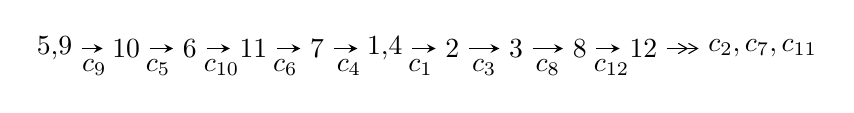
\begin{tikzpicture}[x=23pt, y=7pt]
	% node
	\node (A0) at (-1/8, 0) {5,9};
	\node (A1) at (1, 0) {10};
	\node (A2) at (2, 0) {6};
	\node (A3) at (3, 0) {11};
	\node (A4) at (4, 0) {7};
	\node (A5) at (81/16, 0) {1,4};
	\node (A6) at (49/8, 0) {2};
	\node (A7) at (57/8, 0) {3};
	\node (A8) at (65/8, 0) {8};
	\node (A9) at (73/8, 0) {12};
	\node (C1) at (1/2, -1) {$c_{9}$};
	\node (C2) at (3/2, -1) {$c_{5}$};
	\node (C3) at (5/2, -1) {$c_{10}$};
	\node (C4) at (7/2, -1) {$c_{6}$};
	\node (C5) at (9/2, -1) {$c_{4}$};
	\node (C6) at (45/8, -1) {$c_{1}$};
	\node (C7) at (53/8, -1) {$c_{3}$};
	\node (C8) at (61/8, -1) {$c_{8}$};
	\node (C9) at (69/8, -1) {$c_{12}$};
	\node (A10) at (11, 0) {$c_{2},c_{7},c_{11}$};

	% edge
	\draw[->,>=stealth]	
	(A0) edge (A1) (A1) edge (A2) (A2) edge (A3) (A3) edge (A4) (A4) edge (A5) (A5) edge (A6) (A6) edge (A7) (A7) edge (A8) (A8) edge (A9) ;
	\draw[->>,>={angle 60}]	
	(A9) edge (A10);
\end{tikzpicture} \\ 

\end{tabular} \\

\footnotetext{
The image of knot diagram is generated by the software ``\textbf{Draw programme}" developed by Andrew Bartholomew(\url{http://www.layer8.co.uk/maths/draw/index.htm\#Running-draw}), where we modified some parts for our purpose(\url{https://github.com/CATsTAILs/LinksPainter}).
}\phantom \\ \newline 
\centering \textbf{Ideals for irreducible components\footnotemark of $X_{\text{par}}$} 
 
\begin{align*}
I^u_{1}&=\langle 
4.98637\times10^{30} u^{53}-5.22392\times10^{30} u^{52}+\cdots+3.76717\times10^{30} b-2.97716\times10^{30},\\
\phantom{I^u_{1}}&\phantom{= \langle  }5.96153\times10^{29} u^{53}-5.96332\times10^{30} u^{52}+\cdots+3.76717\times10^{30} a-1.91291\times10^{30},\;u^{54}-2 u^{53}+\cdots- u+1\rangle \\
I^u_{2}&=\langle 
b+1,\;a-1,\;u+1\rangle \\
\\
\end{align*}
\raggedright * 2 irreducible components of $\dim_{\mathbb{C}}=0$, with total 55 representations.\\
\footnotetext{All coefficients of polynomials are rational numbers. But the coefficients are sometimes approximated in decimal forms when there is not enough margin.}
\newpage
\renewcommand{\arraystretch}{1}
\centering \section*{I. $I^u_{1}= \langle 4.99\times10^{30} u^{53}-5.22\times10^{30} u^{52}+\cdots+3.77\times10^{30} b-2.98\times10^{30},\;5.96\times10^{29} u^{53}-5.96\times10^{30} u^{52}+\cdots+3.77\times10^{30} a-1.91\times10^{30},\;u^{54}-2 u^{53}+\cdots- u+1 \rangle$}
\flushleft \textbf{(i) Arc colorings}\\
\begin{tabular}{m{7pt} m{180pt} m{7pt} m{180pt} }
\flushright $a_{5}=$&$\begin{pmatrix}0\\u\end{pmatrix}$ \\
\flushright $a_{9}=$&$\begin{pmatrix}1\\0\end{pmatrix}$ \\
\flushright $a_{10}=$&$\begin{pmatrix}1\\- u^2\end{pmatrix}$ \\
\flushright $a_{6}=$&$\begin{pmatrix}u\\- u^3+u\end{pmatrix}$ \\
\flushright $a_{11}=$&$\begin{pmatrix}- u^2+1\\u^4-2 u^2\end{pmatrix}$ \\
\flushright $a_{7}=$&$\begin{pmatrix}- u^3+2 u\\u^5-3 u^3+u\end{pmatrix}$ \\
\flushright $a_{1}=$&$\begin{pmatrix}-0.158250 u^{53}+1.58297 u^{52}+\cdots-4.25488 u+0.507784\\-1.32364 u^{53}+1.38670 u^{52}+\cdots-1.95767 u+0.790290\end{pmatrix}$ \\
\flushright $a_{4}=$&$\begin{pmatrix}- u\\u\end{pmatrix}$ \\
\flushright $a_{2}=$&$\begin{pmatrix}-0.325199 u^{53}+1.65590 u^{52}+\cdots-5.74265 u+0.513674\\-1.15669 u^{53}+1.31376 u^{52}+\cdots-0.469892 u+0.784399\end{pmatrix}$ \\
\flushright $a_{3}=$&$\begin{pmatrix}-0.210151 u^{53}+1.38312 u^{52}+\cdots-5.45196 u+0.243522\\-1.10881 u^{53}+1.16850 u^{52}+\cdots-0.141966 u+0.636692\end{pmatrix}$ \\
\flushright $a_{8}=$&$\begin{pmatrix}0.270302 u^{53}-0.634518 u^{52}+\cdots-9.79695 u+0.917907\\-0.0490456 u^{53}-0.234591 u^{52}+\cdots-5.02262 u+0.936311\end{pmatrix}$ \\
\flushright $a_{12}=$&$\begin{pmatrix}-0.353877 u^{53}+0.509159 u^{52}+\cdots-10.3335 u+1.46507\\-0.614164 u^{53}+0.364566 u^{52}+\cdots-5.18084 u+1.68406\end{pmatrix}$\\&\end{tabular}
\flushleft \textbf{(ii) Obstruction class $= -1$}\\~\\
\flushleft \textbf{(iii) Cusp Shapes $= -0.476022 u^{53}-2.58830 u^{52}+\cdots-14.0755 u-1.06185$}\\~\\
\newpage\renewcommand{\arraystretch}{1}
\flushleft \textbf{(iv) u-Polynomials at the component}\newline \\
\begin{tabular}{m{50pt}|m{274pt}}
Crossings & \hspace{64pt}u-Polynomials at each crossing \\
\hline $$\begin{aligned}c_{1},c_{3}\end{aligned}$$&$\begin{aligned}
&u^{54}-3 u^{53}+\cdots-321 u+25
\end{aligned}$\\
\hline $$\begin{aligned}c_{2}\end{aligned}$$&$\begin{aligned}
&u^{54}+3 u^{53}+\cdots-75 u-75
\end{aligned}$\\
\hline $$\begin{aligned}c_{4},c_{5},c_{6}\\c_{9},c_{10}\end{aligned}$$&$\begin{aligned}
&u^{54}+2 u^{53}+\cdots+u+1
\end{aligned}$\\
\hline $$\begin{aligned}c_{7},c_{12}\end{aligned}$$&$\begin{aligned}
&u^{54}-20 u^{52}+\cdots+3 u+1
\end{aligned}$\\
\hline $$\begin{aligned}c_{8}\end{aligned}$$&$\begin{aligned}
&15(15 u^{54}+126 u^{53}+\cdots+675 u-223)
\end{aligned}$\\
\hline $$\begin{aligned}c_{11}\end{aligned}$$&$\begin{aligned}
&15(15 u^{54}+114 u^{53}+\cdots+155 u-17)
\end{aligned}$\\
\hline
\end{tabular}\\~\\
\newpage\renewcommand{\arraystretch}{1}
\flushleft \textbf{(v) Riley Polynomials at the component}\newline \\
\begin{tabular}{m{50pt}|m{274pt}}
Crossings & \hspace{64pt}Riley Polynomials at each crossing \\
\hline $$\begin{aligned}c_{1},c_{3}\end{aligned}$$&$\begin{aligned}
&y^{54}-33 y^{53}+\cdots-13641 y+625
\end{aligned}$\\
\hline $$\begin{aligned}c_{2}\end{aligned}$$&$\begin{aligned}
&y^{54}-9 y^{53}+\cdots-165825 y+5625
\end{aligned}$\\
\hline $$\begin{aligned}c_{4},c_{5},c_{6}\\c_{9},c_{10}\end{aligned}$$&$\begin{aligned}
&y^{54}-72 y^{53}+\cdots+9 y+1
\end{aligned}$\\
\hline $$\begin{aligned}c_{7},c_{12}\end{aligned}$$&$\begin{aligned}
&y^{54}-40 y^{53}+\cdots+9 y+1
\end{aligned}$\\
\hline $$\begin{aligned}c_{8}\end{aligned}$$&$\begin{aligned}
&225(225 y^{54}-11196 y^{53}+\cdots-230395 y+49729)
\end{aligned}$\\
\hline $$\begin{aligned}c_{11}\end{aligned}$$&$\begin{aligned}
&225(225 y^{54}-15156 y^{53}+\cdots+8581 y+289)
\end{aligned}$\\
\hline
\end{tabular}\\~\\
\newpage\flushleft \textbf{(vi) Complex Volumes and Cusp Shapes}
$$\begin{array}{c|c|c}  
\text{Solutions to }I^u_{1}& \I (\text{vol} + \sqrt{-1}CS) & \text{Cusp shape}\\
 \hline 
\begin{aligned}
u &= -0.954693 + 0.114732 I \\
a &= -1.07360 + 0.95925 I \\
b &= \phantom{-}0.18824 - 1.51024 I\end{aligned}
 & \phantom{-}1.57417 - 1.88622 I & \phantom{-}7.17160 + 3.60080 I \\ \hline\begin{aligned}
u &= -0.954693 - 0.114732 I \\
a &= -1.07360 - 0.95925 I \\
b &= \phantom{-}0.18824 + 1.51024 I\end{aligned}
 & \phantom{-}1.57417 + 1.88622 I & \phantom{-}7.17160 - 3.60080 I \\ \hline\begin{aligned}
u &= -0.820169 + 0.442176 I \\
a &= \phantom{-}1.36851 - 0.53320 I \\
b &= -0.737742 + 0.980815 I\end{aligned}
 & \phantom{-}1.107040 - 0.620193 I & \phantom{-}11.81390 + 3.24095 I \\ \hline\begin{aligned}
u &= -0.820169 - 0.442176 I \\
a &= \phantom{-}1.36851 + 0.53320 I \\
b &= -0.737742 - 0.980815 I\end{aligned}
 & \phantom{-}1.107040 + 0.620193 I & \phantom{-}11.81390 - 3.24095 I \\ \hline\begin{aligned}
u &= -1.052830 + 0.228694 I \\
a &= -0.085060 - 0.679778 I \\
b &= \phantom{-}0.378348 - 0.402776 I\end{aligned}
 & \phantom{-}2.57681 - 6.14024 I & \phantom{-0.000000 } 0 \\ \hline\begin{aligned}
u &= -1.052830 - 0.228694 I \\
a &= -0.085060 + 0.679778 I \\
b &= \phantom{-}0.378348 + 0.402776 I\end{aligned}
 & \phantom{-}2.57681 + 6.14024 I & \phantom{-0.000000 } 0 \\ \hline\begin{aligned}
u &= \phantom{-}0.903461 + 0.179518 I \\
a &= \phantom{-}1.46868 + 0.05196 I \\
b &= -0.282897 - 1.203480 I\end{aligned}
 & -2.49578 + 3.75084 I & \phantom{-0.000000 } 0. - 6.34793 I \\ \hline\begin{aligned}
u &= \phantom{-}0.903461 - 0.179518 I \\
a &= \phantom{-}1.46868 - 0.05196 I \\
b &= -0.282897 + 1.203480 I\end{aligned}
 & -2.49578 - 3.75084 I & \phantom{-0.000000 -}0. + 6.34793 I \\ \hline\begin{aligned}
u &= \phantom{-}0.909362\phantom{ +0.000000I} \\
a &= \phantom{-}3.13396\phantom{ +0.000000I} \\
b &= -1.83771\phantom{ +0.000000I}\end{aligned}
 & \phantom{-}0.433211\phantom{ +0.000000I} & \phantom{-}12.4360\phantom{ +0.000000I} \\ \hline\begin{aligned}
u &= \phantom{-}1.105440 + 0.194944 I \\
a &= -0.386284 - 0.500062 I \\
b &= -0.0018704 - 0.1304650 I\end{aligned}
 & \phantom{-}5.87997 + 2.18326 I & \phantom{-0.000000 } 0\\
 \hline 
 \end{array}$$\newpage$$\begin{array}{c|c|c}  
\text{Solutions to }I^u_{1}& \I (\text{vol} + \sqrt{-1}CS) & \text{Cusp shape}\\
 \hline 
\begin{aligned}
u &= \phantom{-}1.105440 - 0.194944 I \\
a &= -0.386284 + 0.500062 I \\
b &= -0.0018704 + 0.1304650 I\end{aligned}
 & \phantom{-}5.87997 - 2.18326 I & \phantom{-0.000000 } 0 \\ \hline\begin{aligned}
u &= \phantom{-}1.054560 + 0.387125 I \\
a &= -1.75458 - 0.73634 I \\
b &= \phantom{-}0.99610 + 1.48113 I\end{aligned}
 & \phantom{-}3.53124 + 6.84405 I & \phantom{-0.000000 } 0 \\ \hline\begin{aligned}
u &= \phantom{-}1.054560 - 0.387125 I \\
a &= -1.75458 + 0.73634 I \\
b &= \phantom{-}0.99610 - 1.48113 I\end{aligned}
 & \phantom{-}3.53124 - 6.84405 I & \phantom{-0.000000 } 0 \\ \hline\begin{aligned}
u &= -1.092340 + 0.372866 I \\
a &= \phantom{-}1.85396 - 0.88170 I \\
b &= -0.91541 + 1.72790 I\end{aligned}
 & -1.45842 - 12.26440 I & \phantom{-0.000000 } 0 \\ \hline\begin{aligned}
u &= -1.092340 - 0.372866 I \\
a &= \phantom{-}1.85396 + 0.88170 I \\
b &= -0.91541 - 1.72790 I\end{aligned}
 & -1.45842 + 12.26440 I & \phantom{-0.000000 } 0 \\ \hline\begin{aligned}
u &= \phantom{-}0.455278 + 0.634993 I \\
a &= -1.262020 - 0.389416 I \\
b &= \phantom{-}0.003555 + 1.381020 I\end{aligned}
 & -5.45797 - 4.61873 I & -0.99770 + 3.60735 I \\ \hline\begin{aligned}
u &= \phantom{-}0.455278 - 0.634993 I \\
a &= -1.262020 + 0.389416 I \\
b &= \phantom{-}0.003555 - 1.381020 I\end{aligned}
 & -5.45797 + 4.61873 I & -0.99770 - 3.60735 I \\ \hline\begin{aligned}
u &= -0.748769\phantom{ +0.000000I} \\
a &= -2.10016\phantom{ +0.000000I} \\
b &= -0.0211096\phantom{ +0.000000I}\end{aligned}
 & -3.87941\phantom{ +0.000000I} & -0.406540\phantom{ +0.000000I} \\ \hline\begin{aligned}
u &= \phantom{-}0.318419 + 0.649836 I \\
a &= -0.662849 + 0.251720 I \\
b &= \phantom{-}0.44752 + 1.63240 I\end{aligned}
 & -5.85021 + 8.79187 I & -1.25205 - 7.85625 I \\ \hline\begin{aligned}
u &= \phantom{-}0.318419 - 0.649836 I \\
a &= -0.662849 - 0.251720 I \\
b &= \phantom{-}0.44752 - 1.63240 I\end{aligned}
 & -5.85021 - 8.79187 I & -1.25205 + 7.85625 I\\
 \hline 
 \end{array}$$\newpage$$\begin{array}{c|c|c}  
\text{Solutions to }I^u_{1}& \I (\text{vol} + \sqrt{-1}CS) & \text{Cusp shape}\\
 \hline 
\begin{aligned}
u &= -0.221871 + 0.671219 I \\
a &= \phantom{-}0.335155 + 0.012761 I \\
b &= -0.34810 + 1.38867 I\end{aligned}
 & -0.45577 - 3.26840 I & \phantom{-}4.20658 + 8.69995 I \\ \hline\begin{aligned}
u &= -0.221871 - 0.671219 I \\
a &= \phantom{-}0.335155 - 0.012761 I \\
b &= -0.34810 - 1.38867 I\end{aligned}
 & -0.45577 + 3.26840 I & \phantom{-}4.20658 - 8.69995 I \\ \hline\begin{aligned}
u &= -1.290900 + 0.340769 I \\
a &= \phantom{-}1.31057 - 0.77757 I \\
b &= -0.532843 + 0.817367 I\end{aligned}
 & \phantom{-}0.033603 + 1.175310 I & \phantom{-0.000000 } 0 \\ \hline\begin{aligned}
u &= -1.290900 - 0.340769 I \\
a &= \phantom{-}1.31057 + 0.77757 I \\
b &= -0.532843 - 0.817367 I\end{aligned}
 & \phantom{-}0.033603 - 1.175310 I & \phantom{-0.000000 } 0 \\ \hline\begin{aligned}
u &= -0.478853 + 0.294895 I \\
a &= \phantom{-}0.927174 - 0.540157 I \\
b &= -0.241342 + 0.376066 I\end{aligned}
 & \phantom{-}1.006850 - 0.374600 I & \phantom{-}9.52818 + 2.20824 I \\ \hline\begin{aligned}
u &= -0.478853 - 0.294895 I \\
a &= \phantom{-}0.927174 + 0.540157 I \\
b &= -0.241342 - 0.376066 I\end{aligned}
 & \phantom{-}1.006850 + 0.374600 I & \phantom{-}9.52818 - 2.20824 I \\ \hline\begin{aligned}
u &= \phantom{-}0.299222 + 0.419209 I \\
a &= -0.97060 - 1.29997 I \\
b &= -0.383803 + 0.085272 I\end{aligned}
 & -1.63498 + 3.92306 I & \phantom{-}0.88103 - 8.15922 I \\ \hline\begin{aligned}
u &= \phantom{-}0.299222 - 0.419209 I \\
a &= -0.97060 + 1.29997 I \\
b &= -0.383803 - 0.085272 I\end{aligned}
 & -1.63498 - 3.92306 I & \phantom{-}0.88103 + 8.15922 I \\ \hline\begin{aligned}
u &= \phantom{-}0.238190 + 0.367958 I \\
a &= \phantom{-}0.400758 - 0.042252 I \\
b &= \phantom{-}0.692395 + 0.425963 I\end{aligned}
 & -1.72767 - 1.34489 I & \phantom{-}0.52459 - 1.53353 I \\ \hline\begin{aligned}
u &= \phantom{-}0.238190 - 0.367958 I \\
a &= \phantom{-}0.400758 + 0.042252 I \\
b &= \phantom{-}0.692395 - 0.425963 I\end{aligned}
 & -1.72767 + 1.34489 I & \phantom{-}0.52459 + 1.53353 I\\
 \hline 
 \end{array}$$\newpage$$\begin{array}{c|c|c}  
\text{Solutions to }I^u_{1}& \I (\text{vol} + \sqrt{-1}CS) & \text{Cusp shape}\\
 \hline 
\begin{aligned}
u &= -0.089832 + 0.399750 I \\
a &= \phantom{-}0.23684 - 2.50659 I \\
b &= \phantom{-}0.195200 - 1.035880 I\end{aligned}
 & -5.47596 - 1.75188 I & -7.48810 + 4.25133 I \\ \hline\begin{aligned}
u &= -0.089832 - 0.399750 I \\
a &= \phantom{-}0.23684 + 2.50659 I \\
b &= \phantom{-}0.195200 + 1.035880 I\end{aligned}
 & -5.47596 + 1.75188 I & -7.48810 - 4.25133 I \\ \hline\begin{aligned}
u &= -0.397661\phantom{ +0.000000I} \\
a &= -2.03586\phantom{ +0.000000I} \\
b &= -1.12513\phantom{ +0.000000I}\end{aligned}
 & -4.03946\phantom{ +0.000000I} & \phantom{-}8.30440\phantom{ +0.000000I} \\ \hline\begin{aligned}
u &= \phantom{-}1.68917\phantom{ +0.000000I} \\
a &= \phantom{-}1.87072\phantom{ +0.000000I} \\
b &= -0.736564\phantom{ +0.000000I}\end{aligned}
 & \phantom{-}5.02402\phantom{ +0.000000I} & \phantom{-0.000000 } 0 \\ \hline\begin{aligned}
u &= -1.70299 + 0.03507 I \\
a &= -1.25795 + 0.67361 I \\
b &= \phantom{-}0.495516 - 1.319840 I\end{aligned}
 & \phantom{-}6.81119 - 4.51765 I & \phantom{-0.000000 } 0 \\ \hline\begin{aligned}
u &= -1.70299 - 0.03507 I \\
a &= -1.25795 - 0.67361 I \\
b &= \phantom{-}0.495516 + 1.319840 I\end{aligned}
 & \phantom{-}6.81119 + 4.51765 I & \phantom{-0.000000 } 0 \\ \hline\begin{aligned}
u &= \phantom{-}0.121737 + 0.263787 I \\
a &= \phantom{-}0.57633 - 2.28178 I \\
b &= \phantom{-}0.358359 - 0.939016 I\end{aligned}
 & -1.69045 + 0.57106 I & -4.72601 + 0.62327 I \\ \hline\begin{aligned}
u &= \phantom{-}0.121737 - 0.263787 I \\
a &= \phantom{-}0.57633 + 2.28178 I \\
b &= \phantom{-}0.358359 + 0.939016 I\end{aligned}
 & -1.69045 - 0.57106 I & -4.72601 - 0.62327 I \\ \hline\begin{aligned}
u &= -1.71294\phantom{ +0.000000I} \\
a &= -3.64511\phantom{ +0.000000I} \\
b &= \phantom{-}2.91465\phantom{ +0.000000I}\end{aligned}
 & \phantom{-}9.89130\phantom{ +0.000000I} & \phantom{-0.000000 } 0 \\ \hline\begin{aligned}
u &= \phantom{-}1.71293 + 0.11942 I \\
a &= -2.01031 - 0.80822 I \\
b &= \phantom{-}1.45413 + 1.05839 I\end{aligned}
 & \phantom{-}10.21160 + 2.85652 I & \phantom{-0.000000 } 0\\
 \hline 
 \end{array}$$\newpage$$\begin{array}{c|c|c}  
\text{Solutions to }I^u_{1}& \I (\text{vol} + \sqrt{-1}CS) & \text{Cusp shape}\\
 \hline 
\begin{aligned}
u &= \phantom{-}1.71293 - 0.11942 I \\
a &= -2.01031 + 0.80822 I \\
b &= \phantom{-}1.45413 - 1.05839 I\end{aligned}
 & \phantom{-}10.21160 - 2.85652 I & \phantom{-0.000000 } 0 \\ \hline\begin{aligned}
u &= \phantom{-}1.71703 + 0.02443 I \\
a &= \phantom{-}1.13619 + 1.52937 I \\
b &= -0.57778 - 1.87863 I\end{aligned}
 & \phantom{-}11.16480 + 2.40805 I & \phantom{-0.000000 } 0 \\ \hline\begin{aligned}
u &= \phantom{-}1.71703 - 0.02443 I \\
a &= \phantom{-}1.13619 - 1.52937 I \\
b &= -0.57778 + 1.87863 I\end{aligned}
 & \phantom{-}11.16480 - 2.40805 I & \phantom{-0.000000 } 0 \\ \hline\begin{aligned}
u &= -1.72389\phantom{ +0.000000I} \\
a &= -8.95841\phantom{ +0.000000I} \\
b &= \phantom{-}8.34748\phantom{ +0.000000I}\end{aligned}
 & \phantom{-}9.78120\phantom{ +0.000000I} & \phantom{-0.000000 } 0 \\ \hline\begin{aligned}
u &= \phantom{-}1.73658 + 0.05830 I \\
a &= \phantom{-}0.267916 - 0.025740 I \\
b &= -0.380396 - 0.762948 I\end{aligned}
 & \phantom{-}12.5688 + 7.3202 I & \phantom{-0.000000 } 0 \\ \hline\begin{aligned}
u &= \phantom{-}1.73658 - 0.05830 I \\
a &= \phantom{-}0.267916 + 0.025740 I \\
b &= -0.380396 + 0.762948 I\end{aligned}
 & \phantom{-}12.5688 - 7.3202 I & \phantom{-0.000000 } 0 \\ \hline\begin{aligned}
u &= -1.73758 + 0.10229 I \\
a &= \phantom{-}2.10706 - 1.16433 I \\
b &= -1.44637 + 1.54521 I\end{aligned}
 & \phantom{-}13.4357 - 8.8604 I & \phantom{-0.000000 } 0 \\ \hline\begin{aligned}
u &= -1.73758 - 0.10229 I \\
a &= \phantom{-}2.10706 + 1.16433 I \\
b &= -1.44637 - 1.54521 I\end{aligned}
 & \phantom{-}13.4357 + 8.8604 I & \phantom{-0.000000 } 0 \\ \hline\begin{aligned}
u &= -1.74855 + 0.05158 I \\
a &= \phantom{-}0.1406020 - 0.0077622 I \\
b &= \phantom{-}0.059463 - 0.541387 I\end{aligned}
 & \phantom{-}16.1419 - 3.2325 I & \phantom{-0.000000 } 0 \\ \hline\begin{aligned}
u &= -1.74855 - 0.05158 I \\
a &= \phantom{-}0.1406020 + 0.0077622 I \\
b &= \phantom{-}0.059463 + 0.541387 I\end{aligned}
 & \phantom{-}16.1419 + 3.2325 I & \phantom{-0.000000 } 0\\
 \hline 
 \end{array}$$\newpage$$\begin{array}{c|c|c}  
\text{Solutions to }I^u_{1}& \I (\text{vol} + \sqrt{-1}CS) & \text{Cusp shape}\\
 \hline 
\begin{aligned}
u &= \phantom{-}1.74671 + 0.09995 I \\
a &= -2.04887 - 1.38157 I \\
b &= \phantom{-}1.28385 + 1.80212 I\end{aligned}
 & \phantom{-}8.6391 + 14.2502 I & \phantom{-0.000000 } 0 \\ \hline\begin{aligned}
u &= \phantom{-}1.74671 - 0.09995 I \\
a &= -2.04887 + 1.38157 I \\
b &= \phantom{-}1.28385 - 1.80212 I\end{aligned}
 & \phantom{-}8.6391 - 14.2502 I & \phantom{-0.000000 } 0 \\ \hline\begin{aligned}
u &= \phantom{-}1.76453\phantom{ +0.000000I} \\
a &= -0.974558\phantom{ +0.000000I} \\
b &= \phantom{-}0.804257\phantom{ +0.000000I}\end{aligned}
 & \phantom{-}11.7892\phantom{ +0.000000I} & \phantom{-0.000000 } 0 \\ \hline\begin{aligned}
u &= \phantom{-}1.78233\phantom{ +0.000000I} \\
a &= -0.925833\phantom{ +0.000000I} \\
b &= \phantom{-}0.645888\phantom{ +0.000000I}\end{aligned}
 & \phantom{-}11.7819\phantom{ +0.000000I} & \phantom{-0.000000 } 0\\
 \hline 
 \end{array}$$\newpage\newpage\renewcommand{\arraystretch}{1}
\centering \section*{II. $I^u_{2}= \langle b+1,\;a-1,\;u+1 \rangle$}
\flushleft \textbf{(i) Arc colorings}\\
\begin{tabular}{m{7pt} m{180pt} m{7pt} m{180pt} }
\flushright $a_{5}=$&$\begin{pmatrix}0\\-1\end{pmatrix}$ \\
\flushright $a_{9}=$&$\begin{pmatrix}1\\0\end{pmatrix}$ \\
\flushright $a_{10}=$&$\begin{pmatrix}1\\-1\end{pmatrix}$ \\
\flushright $a_{6}=$&$\begin{pmatrix}-1\\0\end{pmatrix}$ \\
\flushright $a_{11}=$&$\begin{pmatrix}0\\-1\end{pmatrix}$ \\
\flushright $a_{7}=$&$\begin{pmatrix}-1\\1\end{pmatrix}$ \\
\flushright $a_{1}=$&$\begin{pmatrix}1\\-1\end{pmatrix}$ \\
\flushright $a_{4}=$&$\begin{pmatrix}1\\-1\end{pmatrix}$ \\
\flushright $a_{2}=$&$\begin{pmatrix}1\\-1\end{pmatrix}$ \\
\flushright $a_{3}=$&$\begin{pmatrix}1\\-1\end{pmatrix}$ \\
\flushright $a_{8}=$&$\begin{pmatrix}0\\1\end{pmatrix}$ \\
\flushright $a_{12}=$&$\begin{pmatrix}1\\-2\end{pmatrix}$\\&\end{tabular}
\flushleft \textbf{(ii) Obstruction class $= -1$}\\~\\
\flushleft \textbf{(iii) Cusp Shapes $= 6$}\\~\\
\newpage\renewcommand{\arraystretch}{1}
\flushleft \textbf{(iv) u-Polynomials at the component}\newline \\
\begin{tabular}{m{50pt}|m{274pt}}
Crossings & \hspace{64pt}u-Polynomials at each crossing \\
\hline $$\begin{aligned}c_{1},c_{2},c_{3}\end{aligned}$$&$\begin{aligned}
&u
\end{aligned}$\\
\hline $$\begin{aligned}c_{4},c_{5},c_{6}\\c_{7},c_{8},c_{9}\\c_{10},c_{12}\end{aligned}$$&$\begin{aligned}
&u-1
\end{aligned}$\\
\hline $$\begin{aligned}c_{11}\end{aligned}$$&$\begin{aligned}
&u+1
\end{aligned}$\\
\hline
\end{tabular}\\~\\
\newpage\renewcommand{\arraystretch}{1}
\flushleft \textbf{(v) Riley Polynomials at the component}\newline \\
\begin{tabular}{m{50pt}|m{274pt}}
Crossings & \hspace{64pt}Riley Polynomials at each crossing \\
\hline $$\begin{aligned}c_{1},c_{2},c_{3}\end{aligned}$$&$\begin{aligned}
&y
\end{aligned}$\\
\hline $$\begin{aligned}c_{4},c_{5},c_{6}\\c_{7},c_{8},c_{9}\\c_{10},c_{11},c_{12}\end{aligned}$$&$\begin{aligned}
&y-1
\end{aligned}$\\
\hline
\end{tabular}\\~\\
\newpage\flushleft \textbf{(vi) Complex Volumes and Cusp Shapes}
$$\begin{array}{c|c|c}  
\text{Solutions to }I^u_{2}& \I (\text{vol} + \sqrt{-1}CS) & \text{Cusp shape}\\
 \hline 
\begin{aligned}
u &= -1.00000\phantom{ +0.000000I} \\
a &= \phantom{-}1.00000\phantom{ +0.000000I} \\
b &= -1.00000\phantom{ +0.000000I}\end{aligned}
 & \phantom{-}1.64493\phantom{ +0.000000I} & \phantom{-}6.00000\phantom{ +0.000000I}\\
 \hline 
 \end{array}$$\newpage
\newpage\renewcommand{\arraystretch}{1}
\centering \section*{ III. u-Polynomials}
\begin{tabular}{m{50pt}|m{274pt}}
Crossings & \hspace{64pt}u-Polynomials at each crossing \\
\hline $$\begin{aligned}c_{1},c_{3}\end{aligned}$$&$\begin{aligned}
&u(u^{54}-3 u^{53}+\cdots-321 u+25)
\end{aligned}$\\
\hline $$\begin{aligned}c_{2}\end{aligned}$$&$\begin{aligned}
&u(u^{54}+3 u^{53}+\cdots-75 u-75)
\end{aligned}$\\
\hline $$\begin{aligned}c_{4},c_{5},c_{6}\\c_{9},c_{10}\end{aligned}$$&$\begin{aligned}
&(u-1)(u^{54}+2 u^{53}+\cdots+u+1)
\end{aligned}$\\
\hline $$\begin{aligned}c_{7},c_{12}\end{aligned}$$&$\begin{aligned}
&(u-1)(u^{54}-20 u^{52}+\cdots+3 u+1)
\end{aligned}$\\
\hline $$\begin{aligned}c_{8}\end{aligned}$$&$\begin{aligned}
&15(u-1)(15 u^{54}+126 u^{53}+\cdots+675 u-223)
\end{aligned}$\\
\hline $$\begin{aligned}c_{11}\end{aligned}$$&$\begin{aligned}
&15(u+1)(15 u^{54}+114 u^{53}+\cdots+155 u-17)
\end{aligned}$\\
\hline
\end{tabular}\newpage\renewcommand{\arraystretch}{1}
\centering \section*{ IV. Riley Polynomials}
\begin{tabular}{m{50pt}|m{274pt}}
Crossings & \hspace{64pt}Riley Polynomials at each crossing \\
\hline $$\begin{aligned}c_{1},c_{3}\end{aligned}$$&$\begin{aligned}
&y(y^{54}-33 y^{53}+\cdots-13641 y+625)
\end{aligned}$\\
\hline $$\begin{aligned}c_{2}\end{aligned}$$&$\begin{aligned}
&y(y^{54}-9 y^{53}+\cdots-165825 y+5625)
\end{aligned}$\\
\hline $$\begin{aligned}c_{4},c_{5},c_{6}\\c_{9},c_{10}\end{aligned}$$&$\begin{aligned}
&(y-1)(y^{54}-72 y^{53}+\cdots+9 y+1)
\end{aligned}$\\
\hline $$\begin{aligned}c_{7},c_{12}\end{aligned}$$&$\begin{aligned}
&(y-1)(y^{54}-40 y^{53}+\cdots+9 y+1)
\end{aligned}$\\
\hline $$\begin{aligned}c_{8}\end{aligned}$$&$\begin{aligned}
&225(y-1)(225 y^{54}-11196 y^{53}+\cdots-230395 y+49729)
\end{aligned}$\\
\hline $$\begin{aligned}c_{11}\end{aligned}$$&$\begin{aligned}
&225(y-1)(225 y^{54}-15156 y^{53}+\cdots+8581 y+289)
\end{aligned}$\\
\hline
\end{tabular}
\vskip 2pc
\end{document}